\chapter{结语与展望}\label{ch:epilogue}

\epigraph{\textit{抽象的目的不是模糊，而是创造一个新的语义层次，在这个语义层次上可以绝对精确。}}{Edsger W.\ Dijkstra}

全书各章都在研究同一个问题。给定一种变换，概率质量怎样移动？又怎样反转、逼近或利用这一过程来生成数据？本章先回顾贯穿全书的变量变换原理（\Cref{sec:epilogue-backbone}），再用马尔可夫转移核和连续时间马尔可夫链说明如何把同一思路推广到离散状态空间（\Cref{sec:epilogue-discrete}），最后讨论它对其他生成模型的启发（\Cref{sec:epilogue-closing}）。


\chapterlearning{

  \item 将概率传输解释为底层的共同原理
  本书中开发的生成建模框架；

  \item 连接连续空间中的概率演化，通过
  连续性和福克尔-普朗克方程及其有限状态对应项，
  主方程；

  \item 解释逆向建模在离散状态空间中如何变化，其中
  转移核、概率比和跳跃率取代普通的
  欧几里分数数和速度场；

  \item 比较变分、分数/比率和流程视角
  连续和离散的状态空间，确定什么仍然是共同的和
  有什么变化。

}{本章是结语而不是新方法章节。将其读作
综合：关注哪些原则保持不变，哪些数学
当从连续状态空间移动到离散状态空间时，对象必须发生变化。}

\clearpage
\newpage

\section{密度传输的核心框架}\label{sec:epilogue-backbone}

在本书中，我们遵循两条密切相关的开发路线。
第一个是 \emph{ 扩散模型本身 }，包括变分、基于分数和基于流的公式，它们提供了关于概率定律如何演化以及如何逆转这种演化以生成的不同数学描述。
第二个是\emph{扩散驱动的快速生成器}，最著名的是流图模型，它建立在相同的传输观点上，但旨在学习更直接和更高效的生成器。
尽管它们在形式上存在差异，但所有这些方法都植根于一个单一的组织思想：生成建模从根本上来说是一个 \emph{ 传输概率质量 } 的问题。从简单的参考分布（例如高斯噪声）开始，我们寻求构建一个逐渐将其连接到复杂数据分布的过程。这种观点很有用，因为它将注意力从单个模型系列转移到一个更基本的问题上：
\emph{当基础样本按规定的动态移动时，概率定律如何演化？}
回答这个问题的数学语言是变量变换公式及其连续时间推广。从这个意义上说，变量变化原理不仅仅是一种技术工具，而是一种技术工具。它是扩散模型及其激发的快速生成器的概念支柱。

\paragraph{A 普通三步结构.}
从高层次来看，本书中研究的方法都遵循相同的简单模式：
\begin{enumerate}[leftmargin=2em]
    \item 定义一个前向过程，逐渐将数据移向简单的参考分布。
    \item 通过适当的规律演化方程了解概率规律在该过程下如何演化。
    \item 学习一种生成机制，可以逆转、近似或以其他方式利用这种演变来生成样本。
\end{enumerate}
不同公式的不同之处在于前向过程的选择、规律演化方程的数学形式以及生成机制的参数化和训练方式。

\paragraph{变量层次结构的变化.}
在 \Cref{app:continuity} 中，我们开发了变量变换公式的系统级进，从确定性双射到随机微分方程。这一进展在这里值得回顾，因为它揭示了以多种形式出现的单一传输原理。

\FloatBarrier 

\begin{figure}[H]
  \centering

  
  \begin{subfigure}{\textwidth}
    \centering
    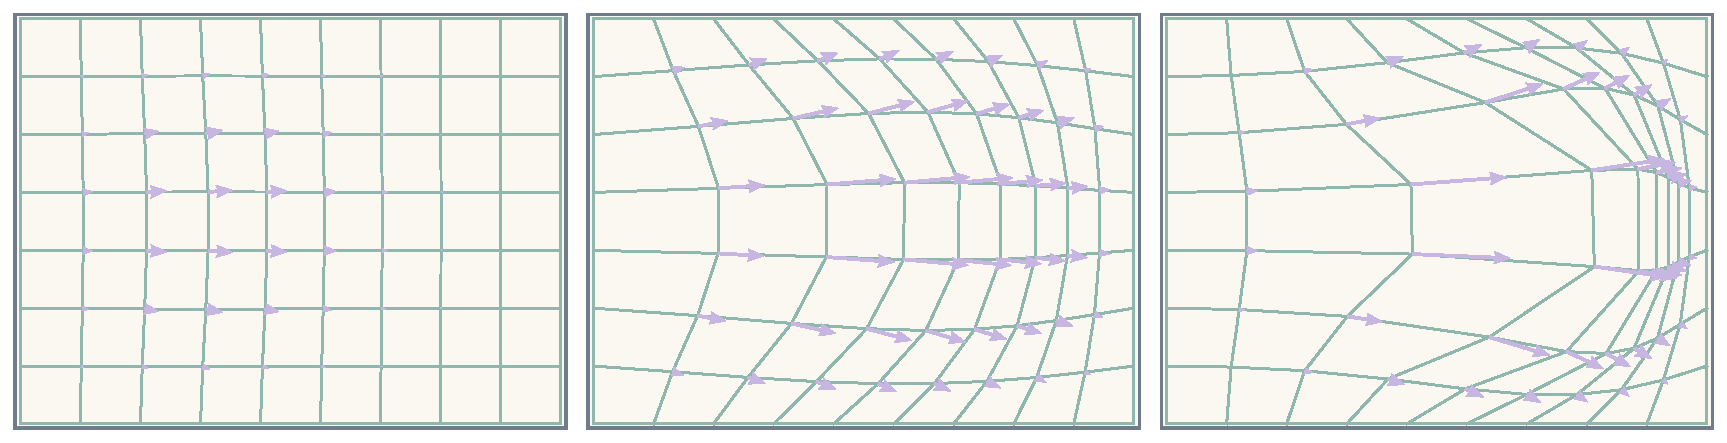
\includegraphics[width=\textwidth]{Images/appendix/vector_field_only.pdf}
        \caption{矢量场插图。箭头代表粒子在空间中移动的速度，相应地使底层网格变形。}
  \end{subfigure}

  \vspace{0.5em} 

  
  \begin{subfigure}{\textwidth}
    \centering
    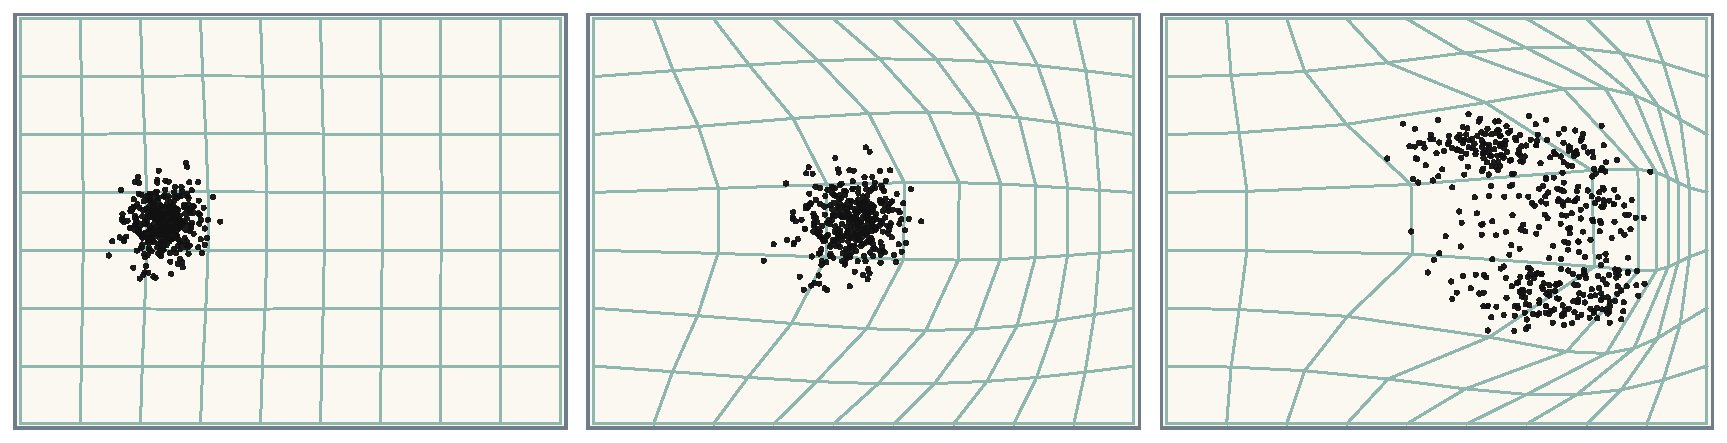
\includegraphics[width=\textwidth]{Images/appendix/particle_cloud.pdf}
    \caption{粒子云动力学。预定义的矢量场生成将粒子从初始状态传输的流。}
  \end{subfigure}

  \vspace{0.5em}

  
  \begin{subfigure}{\textwidth}
    \centering
    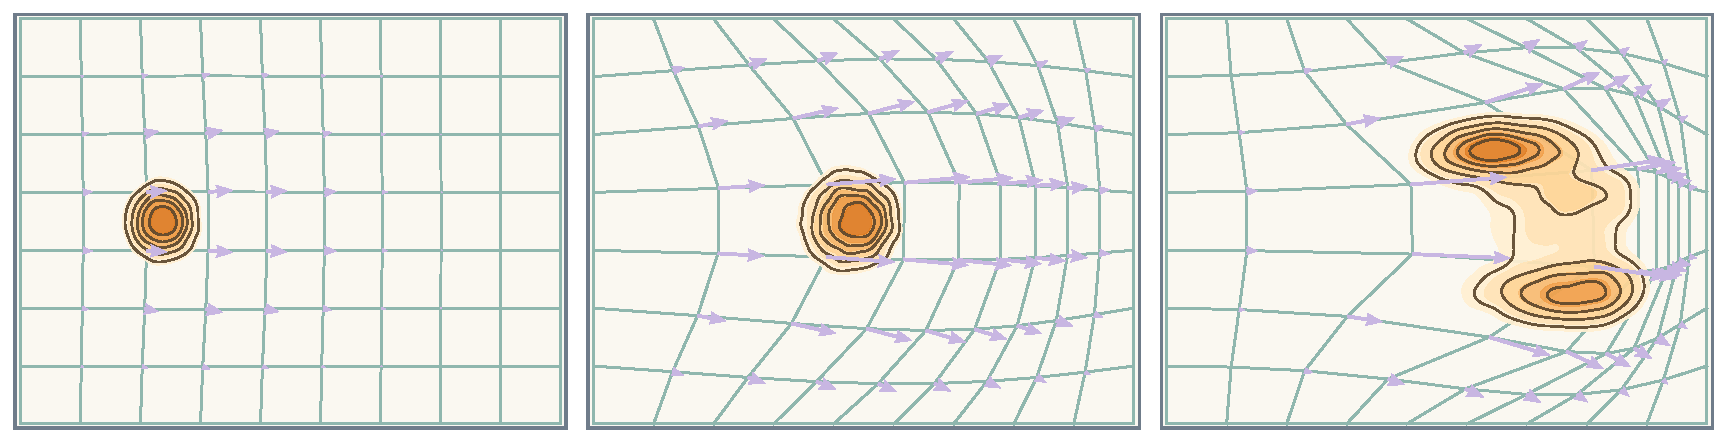
\includegraphics[width=\textwidth]{Images/appendix/vector_field_with_density.pdf}
    \caption{密度演变。当粒子被矢量场平流输送时，密度等值线会相应变形，反映流动如何重塑底层分布。}
  \end{subfigure}

  \caption{\textbfs{矢量场下粒子和密度动力学的图示。}
每列从左到右显示连续的时间快照。 \figcredit{改编自\citet{lipman2024flow}.}
}
  \label{fig:flow-3x3rows}
\end{figure}

\begin{enumerate}[leftmargin=2em]
    \item \textbfs{单双射.}
    平滑可逆映射 $\bPsi:\R^D\to\R^D$ 将密度 $p_0$ 转换为 $p_1$
    \[
    p_1(\rvx_1)
    =
    p_0\bigl(\bPsi^{-1}(\rvx_1)\bigr)
    \left|\det \partial_{\rvx_1}\bPsi^{-1}(\rvx_1)\right|.
    \]
    雅可比行列式记录了体积的局部变化：当映射拉伸空间时，密度减小；当它压缩空间时，密度就会增加。\item \textbfs{组合双射.}
    使用 $\rvx_k=\bPsi_k(\rvx_{k-1})$ 链接多个双射，得到
    \[
    \log p_L(\rvx_L)
    =
    \log p_0(\rvx_0)
    -
    \sum_{k=1}^L
    \log\left|\det \partial_{\rvx_{k-1}}\bPsi_k(\rvx_{k-1})\right|.
    \]
    这是流正常化背后的基本原则。更重要的是，它已经说明了中心信息：一旦指定了粒子运动，密度的演化就会随之而来。

    \item \textbfs{连续时间确定性流 (ODE).}
    取无穷小步长极限可得出连续性方程，
    \[
    \frac{\partial p_t(\rvx)}{\partial t}
    +
    \nabla\cdot\bigl(p_t(\rvx)\,\rvv(\rvx,t)\bigr)
    =
    0,
    \]
    其中粒子根据以下规律演化
    \[
    \frac{\diff \rvx(t)}{\diff t} = \rvv(\rvx(t),t).
    \]
    这就是质量守恒定律的连续时间表达式。概率质量不会被创造或破坏；它只是在速度场 $\rvv$ 下流过空间。

    \item \textbfs{连续时间随机流 (SDE).}
    添加布朗噪声产生福克尔-普朗克方程，
    \[
    \frac{\partial p_t(\rvx)}{\partial t}
    =
    -\nabla\cdot\bigl(\rvv(\rvx,t)\,p_t(\rvx)\bigr)
    +
    \frac{1}{2}g^2(t)\,\Delta p_t(\rvx),
    \]
    这对应于随机动力学
    \[
    \diff\rvx(t) = \rvv(\rvx(t),t)\diff t + g(t)\diff\rvw(t).
    \]
    第一项描述了漂移引起的定向传输，而第二项则描述了噪声引起的随机扩散。
\end{enumerate}

这些不是不相关的公式。
多层变量变化规则是重复确定性变换下传输的离散时间版本。
它的无穷小确定性极限给出了连续性方程。
添加随机扰动可得到福克尔-普朗克方程。
每个级别都扩展了前一个级别，同时保留了相同的基本原理：概率质量守恒，并且概率定律进行调整以反映潜在的动力学如何在空间中移动样本。

从这个角度来看，本书的主要表述更容易放在上下文中。
变分方法描述了通过时间网格上的去噪转变来生成。基于分数的方法与随机动力学一起工作，并学习控制逆时 SDE 的分数场。
基于流的方法与确定性传输一起工作，并学习其诱发的边缘分布遵循规定的中间定律族的速度场。
反过来，快速生成器也建立在相同的主干基础上，但寻求更直接的方法来利用学习到的传输来实现高效采样。

因此，核心要点很简单。
扩散建模不能最好地理解为与一种架构或一种噪声调度相关的单一算法。它是\emph{设计原理}：指定一个前向传输过程，理解概率定律的诱导演化，然后在该结构之上构造一个生成器。一旦这种观点到位，许多看似不同的方法就会成为同一想法的自然变体。

那么一个自然的问题就出现了：这个原理是否超出了连续状态空间？在下一节中，我们将证明确实如此。

\clearpage
\newpage


\section{超越连续状态：离散空间上的概率演化}
\label{sec:epilogue-discrete}到目前为止，本书中的每个模型都在通用结构下运行
假设：生成动力作用的状态存在于
连续欧几里得空间 $\R^D$。 $\rvx$的条目是否代表
像素强度、音频样本或连续潜变量，
数学是一样的：粒子沿着受控制的连续轨迹移动
通过 ODE 或 SDE，概率密度通过连续性或
福克尔-普朗克方程。该框架基于 $\R^D$ 的差分结构：梯度和
散度是通过导数定义的，确定性动力学可以是
由向量场生成的可微轨迹描述。

这种区别是关于建模状态的，而不是关于原始模态的。
离散观测也可以通过首先选择连续代码来处理
和读数。对于原始符号 $a$，令 $\rmE(a)\in\R^d$ 为其代码，
并让 $\rmD$ 将代码映射回符号，或者更一般地映射回
分类分布：
\[
\text{raw discrete symbol } a
\;\xrightarrow{\;\rmE\;}\;
\text{continuous code } \rmE(a)\in\R^d
\;\xrightarrow{\;\rmD\;}\;
\text{discrete readout}.
\]
该表示可以是固定的，例如 one-hot、分类向量或
单值代码~\citep{richemond2022categorical}；
在单射码本上，读出可以是确定性的并且可以满足
$\rmD(\rmE(a))=a$。或者，可以学习表示，
例如令牌嵌入或潜在的自动编码器
\citep{li2022diffusionlm,dieleman2022continuous};那么$\rmD$就是一个有学问的
readout 和 $\rmD\circ\rmE$ 不需要完全可逆。一旦
表示是固定的，扩散是连续状态的：高斯噪声
环境代码空间，或受约束的几何适应连续过程
代码空间，由早期开发的连续机制处理
书。下面研究的有限状态路线是不同的：演化状态
本身仍然是离散的。

本节研究补充案例，其中国家本身
在整个正向和反向过程中保持有限和离散状态。许多数据类型自然适合这种观点：文本是一系列
词汇标记、分子图使用有限的原子和键类型，以及
蛋白质序列是有限字母表上的字符串。在这样一个有限的状态下
空间中不存在从一种状态到另一种状态的典型无穷小位移，
没有通过代币值的平滑轨迹，也没有普通的梯度
国家本身。这就提出了一个自然的问题：
\begin{question}
    如果扩散确实是关于传输概率质量，那么当状态空间有限时，这个想法会变成什么呢？
\end{question}

结构主干保持不变，但数学对象发生了变化。在连续空间中，概率定律在 ODE/SDE 动力学下通过连续性或 福克尔-普朗克方程演化。在有限状态空间中，概率质量根据马尔可夫转移核或跳跃率在状态之间移动，并且定律由有限维守恒定律演化： \emph{主方程}，也称为柯尔莫哥洛夫前向方程。在抽象层面上，这两种设置都遵循相同的方法：

\msg{观察}{}{选择一个前向扰动过程，了解其诱导概率路径，并学习反向传输机制。}

在连续高斯扩散中，这种反向机制表现为高斯反向条件、分数或速度场。在有限状态空间中，它表现为反向转移概率、概率比或跳跃率。这些是不同的数学对象，但它们起着相同的概念作用。本章的目的不是提出一种明确的离散扩散算法。相反，我们制定了一个路线图，随着文献的变化，该路线图应该保持稳定。路线图由用于描述反向传输的对象组织：转换内核、概率比或跳跃率。我们分四个步骤进行：离散时间转换（\Cref{subsec:epilogue-dtmc})，它们的连续时间极限（\Cref{subsec:epilogue-ctmc})，逆向建模的三个视角反映了连续情况的变分、分数/比率和流程观点（\Cref{subsec:epilogue-three-views})，并通过比较突出显示与连续设置的真正不同之处 (\Cref{subsec:epilogue-genuine-diff}).

\subsection{离散时间转移}
\label{subsec:epilogue-dtmc}

设前向过程有 $K$ 个离散类别，其中 $K$ 也计入前向扰动所需的特殊标记，例如掩码。每个状态表示为\emph{独热}列向量 $\rvx\in\{0,1\}^{K}$，其中恰有一个分量等于 $1$。这类向量构成集合\footnote{CTMC 和随机过程文献中的等效公式、标准~\citep{norris1998markov,kelly1979reversibility}，将每个状态表示为标量索引 $x\in\{1,\dots,K\}$，将转换率写为 $[\rmQ_t]_{ij}$，边缘为 $p_t(x)$。这里采用的 one-hot 编码在符号上是等价的，但与离散扩散文献更加一致~\citep{austin2021structured,sahoo2024simple,lou2024discrete}，其中内积如 $\langle\rvx_{\bphi},\rvx\rangle$ 和矩阵——向量积如 $\rmP^{\top}\rvx$ 自然出现在训练目标中。}
\[
\mathcal{V}
= \bigl\{\rvx\in\{0,1\}^{K}:\textstyle\sum_{i=1}^{K}x_i=1\bigr\}
= \{\rve_1,\ldots,\rve_K\}.
\]
记 $\rve_i$ 为第 $i$ 个标准基向量，即类别 $i$ 的独热编码。例如，$\rve_i$ 可以表示一个词元、离散潜在编码、原子类型、键类型或氨基酸。对于文本或蛋白质等序列数据，每个样本由 $N$ 个标记组成，每个标记取自大小为 $K$ 的词表。完整状态空间为 $\mathcal{V}^N$，其大小随序列长度呈指数增长。

许多离散扩散模型在每个位置独立施加前向扰动，单个标记的马尔可夫过程因而是基本单元。我们先讨论单个标记，以说明核心的概率传输机制。对于完整序列，同样的公式适用于整个序列的配置。当各位置的前向扰动相互独立时，给定原始序列的前向转移核可按位置分解为乘积。\footnote{原始数据分布可能含有跨位置的依赖关系，因此扰动所得序列的边缘分布通常无须按位置分解。}
学到的反向模型可以利用不同位置之间的依赖关系。例如，Transformer 或图神经网络可以读取整个受扰样本，再用全局上下文预测局部或全局的反向转移。

\begin{figure}[th!]
    \centering
    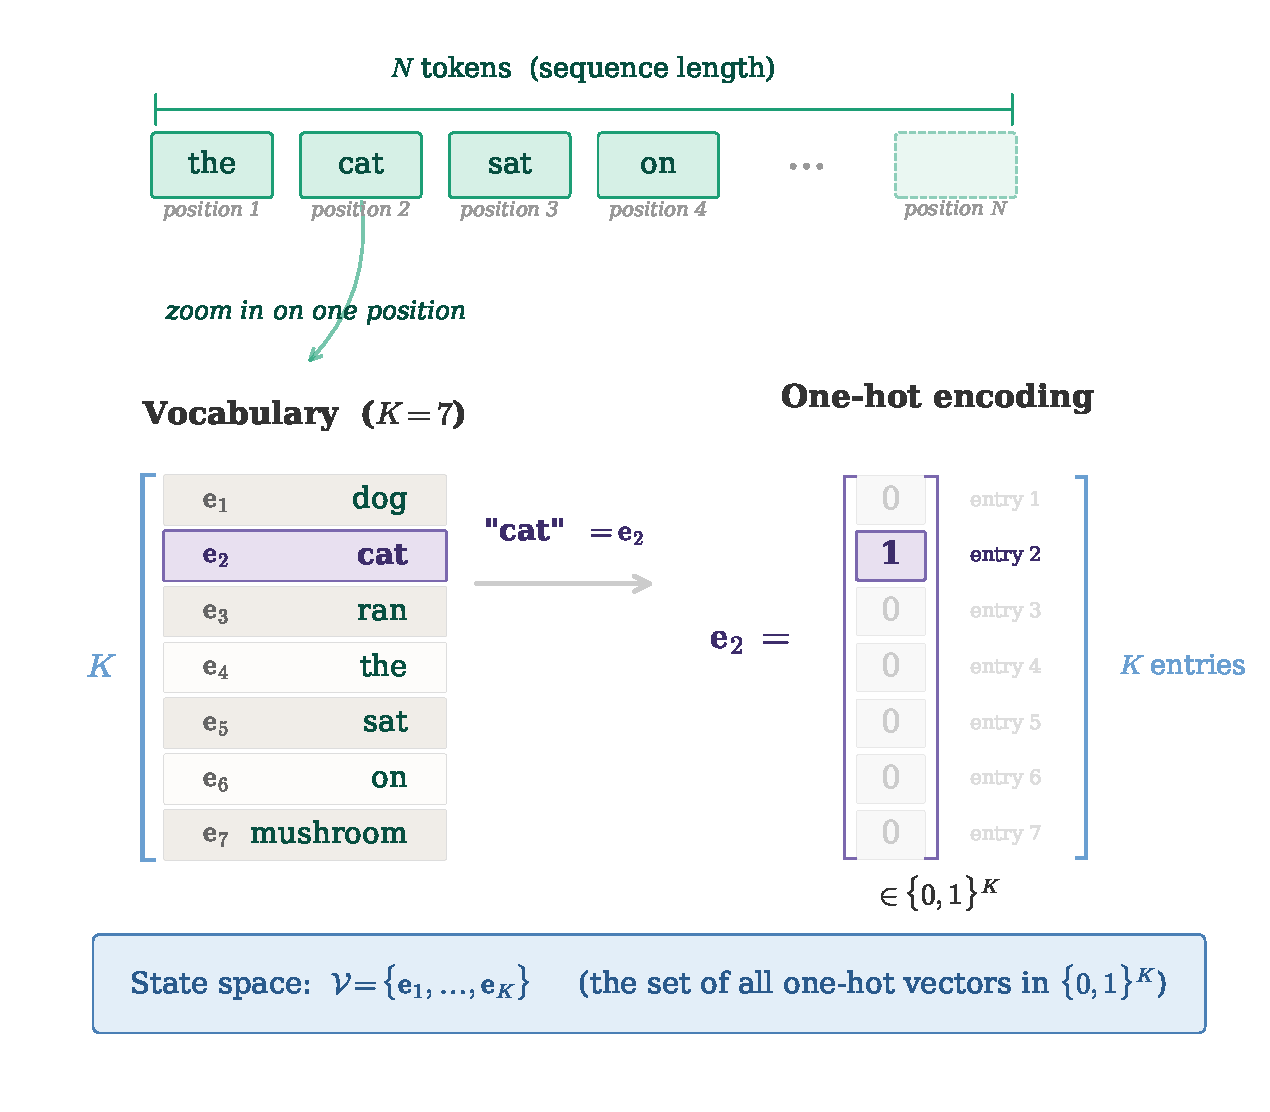
\includegraphics[width=\linewidth]{Images/PartE/fig_notation_overview.pdf}
    \caption{\textbfs{从序列到独热状态。}
    文本或蛋白质序列等数据样本由 $N$ 组成
    令牌，每个令牌都采用大小为 ~$K$ 的有限字母表或词汇表中的值。  本章重点介绍
    $K$ 状态中单个代币的演变。  放大其中一个
    位置，这里是“cat”，token由基向量表示
    $\rve_2$ 并编码为 $\{0,1\}^K$ 中的 one-hot 向量，即
    $K$ 维向量，其第二个条目是 ~$1$ 以及所有其他
    条目为~$0$。  状态空间
    $\mathcal{V}=\{\rvx\in\{0,1\}^K:\sum_{i=1}^K x_i=1\}
    =\{\rve_1,\ldots,\rve_K\}$ 是所有此类 one-hot 向量的集合。
    词汇条目的顺序是任意的并且与以下内容无关
    序列中标记的位置。 \figcredit{由作者使用AI辅助编码创建。}}
    \label{fig:notation-overview}
\end{figure}

在步骤~$k$，系统占据这些$K$状态之一。  我们表示
处于状态 ~$\rve_i$ 的标量概率
\[
p_k(i) := \Pr(\rvx_k=\rve_i),
\qquad i=1,\ldots,K.
\]
收集这些标量概率给出边缘概率向量
\[
\rvp_k
:=
\bigl(p_k(1),\;\dots,\;p_k(K)\bigr)^\top
=
\E[\rvx_k]
\in \Delta^{K-1}\subset\R^K,
\qquad
\sum_{i=1}^K p_k(i)=1,
\]
其中 $\Delta^{K-1}:=\bigl\{\rvp\in\R^K:p_i\geq0,\;
\sum_{i=1}^K p_i=1\bigr\}$ 表示概率单纯形。
等效地，$\Pr(\rvx_k=\rve_i)=p_k(i)$，或简单地
$\rvx_k\sim\mathrm{Cat}(\rvp_k)$。

因此 $\rvp_k$ 是离散随机状态 $\rvx_k$ 的完全定律，而
$p_k(i)$ 是其第 $i$ 标量条目。  在连续时间我们使用相同的
约定：
\[
p_t(i):=\Pr(\rvx_t=\rve_i),
\qquad
\rvp_t:=\bigl(p_t(1),\ldots,p_t(K)\bigr)^\top.
\]
向量 $\rvp_t$ 是密度的离散模拟：它告诉我们如何
总概率质量分布在 $K$ 状态中。

遵循本书中使用的约定，粗体小写字母（$\rvp$, $\rvx$) 表示向量，粗体大写字母 ($\rmP$, $\rmQ$) 表示矩阵，以及未加粗的索引量，例如 $p_k(i)$,
$[\rmP_k]_{ij}$, 和 $[\rmQ_t]_{ij}$ 表示标量条目。未加粗
$p$ 以随机变量为参数，例如
$p(\rvx_{k-1}|\rvx_k)$，表示固定前向过程下的概率质量函数或转移核； $p_{\bphi}$ 表示学习到的逆向模型。系统如何在状态之间移动？单个转换步骤由 \emph{转换矩阵} $\rmP_k \in \R^{K \times K}$。它的条目 $[\rmP_k]_{ij}$ 给出系统当前处于状态的概率~$\rve_i$，移至状态~$\rve_j$ 一步：
\[
[\rmP_k]_{ij} \;=\; \Pr(\rvx_{k+1} = \rve_j | \rvx_k = \rve_i).
\]
因此完整矩阵具有以下结构：
\[
\rmP_k \;=\;
\underbrace{
\begin{pmatrix}
[\rmP_k]_{11} & [\rmP_k]_{12} & \cdots & [\rmP_k]_{1K} \\
[\rmP_k]_{21} & [\rmP_k]_{22} & \cdots & [\rmP_k]_{2K} \\
\vdots & \vdots & \ddots & \vdots \\
[\rmP_k]_{K1} & [\rmP_k]_{K2} & \cdots & [\rmP_k]_{KK}
\end{pmatrix}
}_{\substack{\text{columns: next state } j}}
\quad
\left.
\vphantom{
\begin{pmatrix}
a \\ a \\ \vdots \\ a
\end{pmatrix}
}
\right\}
\text{\footnotesize rows: current state } i.
\]
跨行读取 $i$ 答案：``鉴于系统当前处于状态 $\rve_i$，在每个可能的下一个状态着陆的概率是多少？”因此，每一行都是目的地的概率分布：
\[
[\rmP_k]_{ij} \geq 0
\quad \text{for all } i,j,
\qquad\qquad
\sum_{j=1}^{K} [\rmP_k]_{ij} = 1
\quad \text{for each } i.
\]
非负条件表示每个转移概率都是有效的，行和约束表示所有质量离开状态~$\rve_i$ 考虑到：系统总是在某个地方结束。

\paragraph{分布如何演变。}
有了转移矩阵，我们现在问一个基本问题：系统是否以分布开始 $\rvp_k$，一步后的分布是怎样的？答案来自简单的概率统计。处于状态的概率~$\rve_j$ 转变后到达的总质量~$\rve_j$ 来自所有可能的源状态：
\begin{equation}
p_{k+1}(j) = \sum_{i=1}^K p_k(i)\,[\rmP_k]_{ij}.
\label{eq:discrete-transport-one-step}
\end{equation}
总和中的每一项代表初始状态下的质量~$\rve_i$，按从以下位置跳转的概率加权~$\rve_i$ 至~$\rve_j$。以向量形式，这变成
\[
\rvp_{k+1} = \rmP_k^\top \rvp_k.
\]
等价地，给定当前one-hot状态的下一状态的条件分布~$\rvx_k$ 是
\[
\Pr(\rvx_{k+1} | \rvx_k)
= \mathrm{Cat}(\rvx_{k+1};\,\rmP_k^\top\,\rvx_k),
\]
自 $\rmP_k^\top\,\rve_i$ 提取 $i$第-行~$\rmP_k$，包含状态的转移概率~$\rve_i$。按此规则演化的系统称为 \emph{离散时间马尔可夫链}: 以当前状态为条件 $\rvx_k$，分布
$\rvx_{k+1}$ 不依赖于早期状态。这起到了连续空间中规律演化公式的有限状态作用。那里有一个双射 $\bPsi$ 重塑密度，雅可比行列式补偿局部体积变化。在有限状态空间中，没有要跟踪的体积元素。相反，转移矩阵 $\rmP_k$ 直接指定离开每个源状态并到达每个目的地的概率质量。行和约束保证总概率守恒，就像连续性方程中的散度结构一样。

使用转移矩阵在多个步骤中重复此操作
$\rmP_0, \dots, \rmP_{L-1}$, 产量
\begin{equation*}
\rvp_L = \rmP_{L-1}^\top \cdots \rmP_1^\top \rmP_0^\top\, \rvp_0.
\end{equation*}
这反映了多层变量变换公式
\Cref{eq:cov-multi-layer-nolog}。在连续确定性环境中，密度演化是通过雅可比行列式累积的；这里，概率向量通过连续的马尔可夫算子传播。基本思想是相同的：通过一系列规定的变换来跟踪概率质量。

\paragraph{反转单步。}
考虑到正向机制，很自然地会问如何反转单个转换以进行生成。假设观察到系统处于状态~$\rve_j$ 在步骤中~$k{+}1$。处于状态的概率是多少~$\rve_i$ 在上一步~$k$？这是贝叶斯规则的直接应用：
\begin{align}
\Pr(\rvx_k = \rve_i | \rvx_{k+1} = \rve_j)
= \frac{\Pr(\rvx_{k+1} = \rve_j | \rvx_k = \rve_i)\;\Pr(\rvx_k = \rve_i)}
        {\Pr(\rvx_{k+1} = \rve_j)}  
= [\rmP_k]_{ij}\frac{p_k(i)}{p_{k+1}(j)},
\label{eq:discrete-reverse-kernel}
\end{align}
每当 $p_{k+1}(j)>0$。这是与前向过渡相关的离散时间反向转移核~$\rmP_k$ 与现行边缘法一起。它的形式是直观的：在质量达到状态的所有方式中~$\rve_j$，每个来源~$\rve_i$ 与质量成正比，通过 $p_k(i)$，以及跳跃的可能性有多大 $[\rmP_k]_{ij}$。中的分子和分母 \Cref{eq:discrete-reverse-kernel} 每一个都有明确的解释：
\begin{itemize}[leftmargin=2em]
    \item \textbfs{分子:}
    术语 $[\rmP_k]_{ij}\,p_k(i)$ 是处于状态的联合概率~$\rve_i$ 在步骤中~$k$ 然后跳转到~$\rve_j$ 在步骤中~$k{+}1$.

    \item \textbfs{分母：}
    术语
    \[
    p_{k+1}(j) = \sum_{i'} p_k(i')\,[\rmP_k]_{i'j}
    \]
    是到达状态的总概率~$\rve_j$ 来自任何来源。它用作归一化常数，确保反向概率之和为一~$i$.
\end{itemize}

关键的一点是反向转移核是 \emph{没有} 的矩阵逆 $\rmP_k$。马尔可夫转移可以将多个状态的概率质量合并到一个状态，并且它不需要像线性映射一样可逆。相反，概率逆是贝叶斯逆，它不仅取决于前向转移矩阵，还取决于边缘分布 $\rvp_k$。这正是生成建模面临的困难： $\rvp_k$ 是通过前向过程推送未知数据分布得到的，因此通常无法以封闭形式获得。下面的逆向建模视角可以理解为表示或学习实现贝叶斯逆向所需的缺失信息的不同方式。

\subsection{连续时间极限：主方程}
\label{subsec:epilogue-ctmc}

在连续空间的故事中，将组合双射的步长缩小到零产生了连续性方程（\Cref{subsec:cov-continuity-eq}）。同样的限制思想在这里也适用。当时间步长变得无限小时，离散时间马尔可夫链变成连续时间马尔可夫链（CTMC），并且分布根据主方程演化。

\begin{figure}[th!]
    \centering
    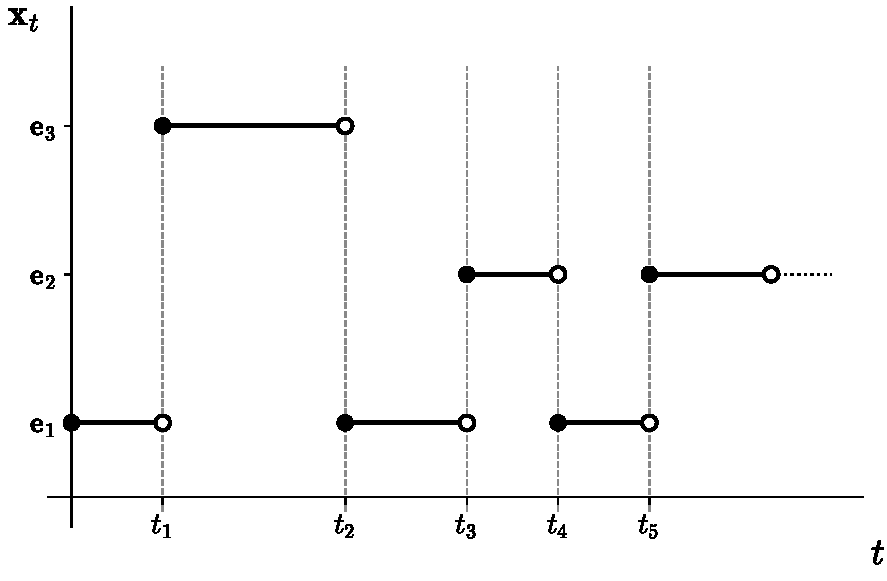
\includegraphics[width=0.8\linewidth]{Images/PartE/ctmc_trajectory.pdf}
    \caption{\textbfs{CTMC 样本路径图示。}
设状态空间为 $\mathcal{V}=\{\rve_1,\rve_2,\rve_3\}$，标记为 $S_1,S_2,S_3$ 在垂直轴上。轨迹是分段常数：过程保持在 $\rvx_t=\rve_i$ 随机保持一段时间，然后瞬间跳转到另一个状态 $\rve_j$ 有时 $t_1,t_2,\ldots$。实心圆圈标记每次跳转后立即占据的状态，空心圆圈标记跳转前的状态，反映右连续约定。虚线部分表示超出显示窗口的继续。这些跳跃时间和目的地由速率矩阵控制 $\rmQ_t$: 来自州 $\rve_i$，进程跳转到 $\rve_j$ ($j\neq i$) 瞬时速率 $[\rmQ_t]_{ij}$.
\figcredit{改编自 \citet{campbell2022continuous}.}}
    \label{fig:ctmc-trajectory}
\end{figure}

\paragraph{无穷小过渡。}
在上一小节中，每个转换矩阵 $\rmP_k$ 描述了时间的完整步骤 $k$ 到时间 $k{+}1$。现在想象一下让这些步骤变得越来越精细。让 $\rmP_{t,\Delta t}$ 表示使系统向前移动一小段持续时间的转移矩阵 $\Delta t$ 开始时间 $t$: 其条目 $[\rmP_{t,\Delta t}]_{ij}$ 是从状态移动的概率~$\rve_i$ 说明~$\rve_j$ 间歇期间
$[t,\,t{+}\Delta t]$.

当 $\Delta t$ 很小，大部分质量保持不变，只有一小部分会跳跃。这意味着 $\rmP_{t,\Delta t}$ 接近恒等式，我们可以将其展开为
\begin{equation}
\rmP_{t,\Delta t}
\;=\; \rmI + \rmQ_t\,\Delta t + \mathcal{O}(\Delta t^2),
\label{eq:generator-expansion}
\end{equation}
其中 $\rmQ_t \in \R^{K \times K}$ 是 \emph{速率矩阵}，也称为生成器，当时 $t$。如果 $\rmQ_t$ 在时间上足够规则，余数可以写为 $\mathcal{O}(\Delta t^2)$ 本地。的条目 $\rmQ_t$ 是瞬时的
\emph{费率} 而不是概率。具体来说：
\begin{itemize}[leftmargin=2em]
    \item $[\rmQ_t]_{ij} \geq 0$ 用于 $i \neq j$: 这是进程从状态跳转的速率~$\rve_i$ 说明~$\rve_j$。乘以 $\Delta t$ 给出短间隔内的前导跳跃概率。
    \item $[\rmQ_t]_{ii} = -\sum_{j \neq i} [\rmQ_t]_{ij}$：对角线条目为负数，记录概率从下列状态流出的总速率~$\rve_i$。这确保了每一行 $\rmQ_t$ 总和为零，这是概率守恒的速率级表达式。\footnote{这直接来自行总和约束 $\rmP_{t,\Delta t}$。由于转移矩阵的每一行总和为 $1$，替换扩展
      $\rmP_{t,\Delta t} = \rmI + \rmQ_t\,\Delta t
      + o(\Delta t)$ 给出
      $1 + \Delta t \sum_{j} [\rmQ_t]_{ij}
      + o(\Delta t) = 1$，这迫使 $\sum_{j} [\rmQ_t]_{ij} = 0$。分离对角线项得出
      $[\rmQ_t]_{ii} = -\sum_{j \neq i} [\rmQ_t]_{ij}$.}
\end{itemize}
读取扩展，从~$\rve_i$ 至
$\rve_j$ 与 $j\neq i$ 在短时间内大约是
$[\rmQ_t]_{ij}\,\Delta t$，而停留在的概率~$\rve_i$ 大约是
$1 - \sum_{j \neq i} [\rmQ_t]_{ij}\,\Delta t$.

\paragraph{主方程。}
随着手中的无限小的转换，连续时间极限立即出现。将展开式代入 \Cref{eq:generator-expansion}
进入 $\rvp_{t+\Delta t} = \rmP_{t,\Delta t}^\top\,\rvp_t$ 并采取
$\Delta t \to 0$ 给出
\begin{mdframed}
\begin{equation}
\frac{\diff}{\diff t}\,\rvp_t = \rmQ_t^\top\,\rvp_t.
\label{eq:master-equation-vector}
\end{equation}
\end{mdframed}
这是 \emph{主方程}，也称为 \emph{柯尔莫哥洛夫前向方程} 用于 CTMC~\citep{norris1998markov}。回想一下 $\rvp_t$ 是概率向量，其 $j$第-条目 $p_t(j)$ 给出处于状态的概率~$\rve_j$ 当时~$t$。写出 $j$第-个组件
\Cref{eq:master-equation-vector} 使含义具体化：
\begin{equation}
\frac{\diff}{\diff t}\,p_t(j)
= \underbrace{\sum_{i \neq j} p_t(i)\,[\rmQ_t]_{ij}}_{\text{inflow: mass arriving from other states}}
\;-\;
\underbrace{p_t(j)\sum_{\ell \neq j} [\rmQ_t]_{j\ell}}_{\text{outflow: mass departing to other states}}.
\label{eq:master-equation-component}
\end{equation}
变化率 $p_t(j)$ 只是流入减去流出。这是用微分方程表示的概率守恒。\paragraph{与连续性方程的比较.}
在连续空间中，连续性方程
\[
\partial_t\,p_t(\rvx) + \nabla \cdot
\big(p_t(\rvx)\,\rvv(\rvx,t)\big) = 0
\]
说密度变化是由概率质量的净通量驱动的
在速度场 $\rvv$ 下。主方程也是这样说的
有限状态语言中的事物：$p_t(j)$ 由于受以下因素控制的净概率通量而发生变化
速率矩阵 $\rmQ_t$。速度场和速率矩阵的作用
类似的结构角色：都规定了概率质量如何
重新分配，并且都强制保护。主要区别是几何上的：在 $\R^D$ 中，质量流过相邻的空间位置；在有限状态空间中，质量沿着转移图的允许边缘跳跃。

\begin{figure}[th!]
    \centering
    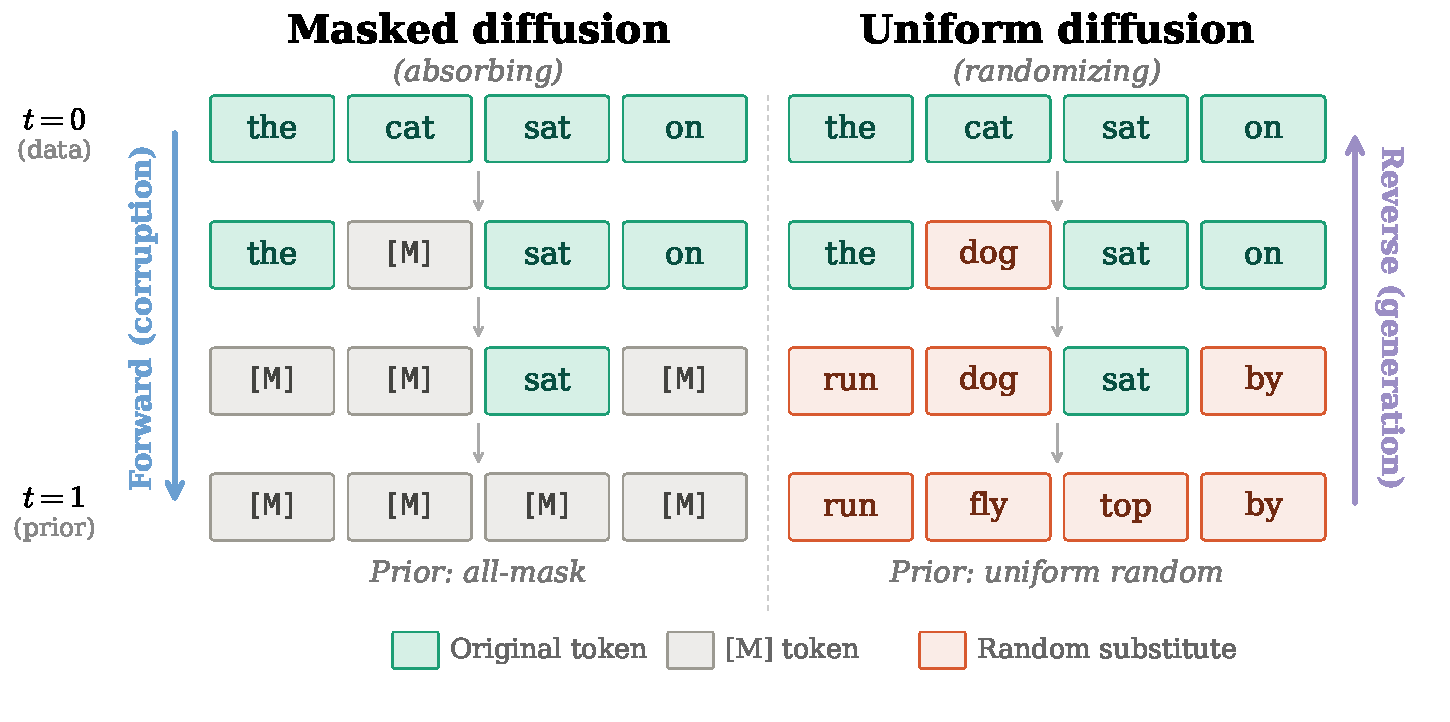
\includegraphics[width=\linewidth]{Images/PartE/masked_vs_uniform_diffusion.pdf}
\caption{\textbfs{ 屏蔽和均匀扩散前向扰动和反向生成的图示。}
此处显示的两个示例承认以下形式的插值边缘
$\Pr(\rvx_t|\rvx_0)=\mathrm{Cat}(\rvx_t;\alpha_t\rvx_0+(1-\alpha_t)\bm{\pi})$，
其中确定了限制先验 $\bm{\pi}$ 和衰减因子 $\alpha_t$
通过选择的远期汇率矩阵。  在掩蔽扩散中，令牌是
吸收到掩模状态，限制先前的$\bm{\pi}=\rvm=\rve_K$。  在
均匀扩散，令牌被重复随机化，限制先验
$\bm{\pi}_{\mathrm{unif}}=\frac{1}{K}\mathbf{1}$。  生成过程从这个简单的参考分布或其有限时间近似出发，逆转所选的前向扰动。
\figcredit{由作者使用AI辅助编码创建。}}
    \label{fig:mask-uniform}
\end{figure}

\paragraph{前向扰动。}
与连续扩散一样，我们需要通过前向过程逐步打散数据分布的结构，使它趋近于易于采样的参考分布。离散扰动在这里起到与连续扩散中高斯加噪相同的作用。扰动应当逐步施加，便于解析处理或数值计算，并在终止时刻 $T$ 基本消除初始数据分布的结构。

可以通过多种方式选择速率矩阵。它可以是统一的、吸收性的、最近邻的、基于图形的、化学结构的、语法感知的或以其他方式适应数据域的。因此，以下两个示例并不意味着详尽的分类法；它们是使机制透明的典型案例。
\subparagraph{掩模扩散（吸收）。} 保留最后一个
      类别作为掩码标记，写作 $\rvm := \rve_K$。  干净的数据
      $\rvx_0$ 占据第一个 $K{-}1$ 类别之一，因此
      $\langle\rvx_0,\rvm\rangle = 0$。  速率矩阵定义如下
      每个普通状态都会转换到掩码状态
      rate~$\beta(t)$，而掩码状态永远不会转换出来：
\[
[\rmQ_t]_{iK}=\beta(t),\qquad
[\rmQ_t]_{ii}=-\beta(t),\qquad
[\rmQ_t]_{ij}=0
\quad
\text{for } i<K,\; j\notin\{i,K\},
\]
和
\[
[\rmQ_t]_{Kj}=0
\quad
\text{for all } j.
\]
      这个想法很简单：每个令牌都独立地替换为
      屏蔽速率为 ~$\beta(t)$，一旦屏蔽，它就会保持屏蔽状态。以干净状态~$\rvx_0$为条件的前向边缘为
      \[
      \Pr(\rvx_t | \rvx_0)
      = \mathrm{Cat}\bigl(\rvx_t;\;
          \alpha_t\,\rvx_0 + (1-\alpha_t)\,\rvm\bigr),
      \]
      其中
      \[
      \alpha_t
      =
      \exp\left(-\int_0^t\beta(s)\,\diff s\right).
      \]
      在时间~$t$，代币等于其干净价值~$\rvx_0$
      概率 ~$\alpha_t$ 并用概率 ~$1-\alpha_t$ 进行掩码。
      随着时间的增加，越来越多的概率质量积累在
      掩码状态。  如果 $\int_0^T\beta(s)\diff s$ 大，则 $\alpha_T$ 小，终端分布接近全掩模参考分布。

\subparagraph{均匀扩散。} 这不是擦除令牌，而是
      过程逐渐使其随机化。  一种方便的连续时间标准化是让令牌以相同的速率跳转到其他每个 $K-1$ 状态：
      \[
      [\rmQ_t]_{ij} = \frac{\beta(t)}{K - 1}
      \quad\text{for } i \neq j,
      \qquad
      [\rmQ_t]_{ii} = -\beta(t).
      \]
      第一个公式表示从状态~$\rve_i$开始，代币跳转
      以相同的瞬时速率到达每个替代状态。  第二个说的是
      离开状态的总速率~$\rve_i$为~$\beta(t)$。

      前向边缘再次采用插值形式
      \[
      \Pr(\rvx_t|\rvx_0)
      = \mathrm{Cat} \bigl(\rvx_t;\;
          \alpha_t\,\rvx_0 + (1-\alpha_t)\,\bm{\pi}_{\mathrm{unif}}
        \bigr),
      \]
      其中
      $\bm{\pi}_{\mathrm{unif}}=\tfrac{1}{K}\mathbf{1}\in\R^K$ 是
      均匀概率向量。  在上述速率标准化下，
      衰减因子是
      \[
      \alpha_t
      =
      \exp\left(
      -\frac{K}{K-1}\int_0^t \beta(s)\,\diff s
      \right).
      \]
      随着时间的推移，重复的随机化会消除结构
      数据分布并将其推向均匀分布
      上~$\mathcal{V}$。

更一般地，正向过程不需要具有简单混合形式
\[
\Pr(\rvx_t|\rvx_0)
= \mathrm{Cat}\bigl(\rvx_t;\;\alpha_t\rvx_0+(1-\alpha_t)\bm{\pi}\bigr).
\]
该形式对于直觉很有用，并且以常见的蒙版和统一形式出现
结构，但马尔可夫定律演化观点更为普遍：
转移矩阵控制离散时间演化，速率矩阵控制
通过主方程进行连续时间演化。结构化离散扩散模型可以使用尊重编辑距离、图邻接性、分子有效性、词汇结构或其他领域知识的转换规则。在所有情况下，相同的原则仍然存在：前向马尔可夫过程定义了一条概率路径，并且一代人学会沿着相反的路径移动。

\subsection{逆向建模的三个视角}
\label{subsec:epilogue-three-views}

一旦正向过程及其演化规律就位，剩下的任务与连续情况下的相同：学习一个反向过程，其边缘分布在反向时间内回溯正向演化，将简单的参考样本转化为数据。在~B部分中，
我们将连续扩散模型分为三个视角：
变分 (\Cref{ch:variational})，基于分数
（\Cref{ch:score-based,ch:score-sde}），以及基于流的
（\Cref{ch:flow-based}）。同样的三向观点也适用于离散环境，但有一个重要的警告：这些不是相互排斥的流派或固定的论文类别。它们是识别必须学习哪些未知对象才能反转概率路径的三种方法。

\paragraph{变分视角：学习逆向转移核。}
在连续状态空间中（见 \Cref{sec:ddpm}），变分视角把扩散模型看作分层潜变量模型。前向过程产生一系列噪声越来越强的潜变量，训练的目标是学习反向转移，逐步去噪。真实的反向转移核 $\Pr(\rvx_{k-1}|\rvx_k)$ 依赖 $\rvx_k$ 的边缘分布，因此涉及未知的数据分布。DDPM 的做法是进一步以干净样本 $\rvx_0$ 为条件。这样，由前向过程得到的后验 $\Pr(\rvx_{k-1}|\rvx_k, \rvx_0)$ 是可以显式写出的高斯分布。定理~\ref{thm:equiv-marginal-kl} 表明，用这个条件后验构造的训练目标，与用边缘反向转移核构造的目标只相差一项与反向模型无关的量。ELBO 因而可以分解为一系列 KL 散度项（见 \Cref{eq:ddpm-diffusion}），每个噪声水平对应一项，用于拟合一个可计算的前向后验。

这一思路也适用于离散状态空间。先从数据分布抽取 $\rvx_0$，再运行固定的前向马尔可夫链，把所得的联合分布记为 $p$，把学习到的反向模型记为 $p_{\bphi}$。考虑一条由独热向量表示的前向扰动链
\[
\rvx_0 \;\xrightarrow{\;\rmP_0\;}\; \rvx_1 \;\xrightarrow{\;\rmP_1\;}\;
\cdots \;\xrightarrow{\;\rmP_{L-1}\;}\; \rvx_L,
\]
其中 $\rvx_0$ 从数据分布中得出 $\rvx_L$ 接近简单的参考分布，例如全掩模或均匀分布。现在，转换是分类的而不是高斯的，但变分结构是相同的：
\begin{itemize}[leftmargin=2em]
    \item 真正的相反 $p(\rvx_{k-1}|\rvx_k)$ 很棘手，因为它取决于步长的边缘~$k$.
    \item 给定 $\rvx_0$ 后，可以用贝叶斯公式计算前向过程的条件后验。
      \[
      p(\rvx_{k-1}|\rvx_k, \rvx_0)
      =
      \frac{p(\rvx_k|\rvx_{k-1})\;p(\rvx_{k-1}|\rvx_0)}
             {p(\rvx_k|\rvx_0)},
      \]
      其中右侧的每个因素都由前向过程确定。
    \item 用条件后验训练与用边缘反向转移核训练，得到的最优反向转移核相同。两个目标只相差一项与 $p_{\bphi}$ 无关的量。
\end{itemize}

示意性地讲，离散扩散 ELBO 包含以下形式的降噪项
\[
\E_{p(\rvx_{0:L})}
 \Big[
\mathcal{D}_{\mathrm{KL}} \big(
  p(\rvx_{k-1}|\rvx_k, \rvx_0)
  \;\|\;
  p_{\bphi}(\rvx_{k-1}|\rvx_k)
\big)
\Big],
\qquad k=1,\ldots,L.
\]
根据具体模型，完整的 ELBO 还包括边界项，例如终端先验项和附近的重建项 $k=0$。关键点是，每个去噪项都要求学习到的反向转移核与由前向扰动确定的易处理的贝叶斯后验相匹配。这里 $p_{\bphi}(\rvx_{k-1}=\rve_i|\rvx_k=\rve_j)$ 表示神经网络参数化反向转移概率：假设系统处于状态~$\rve_j$ 在步骤中~$k$，给出来自状态的概率~$\rve_i$ 在步骤中~$k{-}1$。对于每个固定~$\rve_j$，这些值形成了先前状态的分类分布。与连续 DDPM 的主要形式区别在于这些 KL 散度
是离散状态上的有限和而不是封闭式高斯
表达式。这反映了高斯分布的一个特殊性质：同一变量中两个高斯密度的乘积与另一个高斯密度成正比。在连续 DDPM 中，
前向后验是通过乘以高斯因子计算的，因此结果本身就是高斯的，并且
KL 散度简化为一个简单的代数表达式，涉及
仅均值和协方差 (\Cref{sec:ddpm})。在离散设置中，
贝叶斯规则产生的是分类分布，每个 KL 项都是状态的总和。这个总和是精确的并且概念上简单，但是对于大词汇表或完整序列空间，它可能需要结构、因式分解、子采样或专门的参数化。

关于参数化的一个实际问题也值得注意。 ELBO 询问
学习反向转移核 $p_{\bphi}(\rvx_{k-1}|\rvx_k)$ 来匹配贝叶斯
后验，但它不会强制对其进行一种独特的神经参数化
内核。一种常见的选择是干净状态，或 $x_0$ 预测，
参数化。精确的边缘逆核满足恒等式
\[
p(\rvx_{k-1}|\rvx_k)
=
\sum_{a}
p(\rvx_{k-1}|\rvx_k,\rvx_0=\rve_a)\,
p(\rvx_0=\rve_a|\rvx_k),
\]
其中总和超过有效的清洁类别。这简直就是边缘化
超过未知的清洁状态。由于后验 $p(\rvx_0|\rvx_k)$ 取决于
数据分布，它不以封闭形式提供。因此，模型可以
预测干净状态分布 $\widehat p_{\bphi}(\rvx_0|\rvx_k)$ 并使用
它来定义
\[
p_{\bphi}(\rvx_{k-1}|\rvx_k)
:=
\sum_{a}
p(\rvx_{k-1}|\rvx_k,\rvx_0=\rve_a)\,
\widehat p_{\bphi}(\rvx_0=\rve_a|\rvx_k).
\]
如果 $\widehat p_{\bphi}(\rvx_0|\rvx_k)$ 等于真实后验
$p(\rvx_0|\rvx_k)$，这种混合物将恢复精确的反向转移核。在
实践中，这是将学到的反向转换与已知的联系起来的有用方法
向前向后。

这种干净状态参数化在多项式/D3PM 式中很常见
离散时间扩散模型~\citep{hoogeboom2021argmax,austin2021structured}，
但这不是离散扩散的定义。 D3PM 本身指出，
可以直接预测反向逻辑，后来的模型使用其他
针对前向过程定制的结构化参数化
\citep{sahoo2024simple}。因此，清洁状态预测应被视为一种
变分视角的重要参数化，而不是唯一的方法
模拟逆过程。

\paragraph{分数/比率视角：学习局部概率比较。}
在连续情况下（\Cref{ch:score-based,ch:score-sde}），
基于分数的观点从一个简单的问题开始：给定一个损坏的
样品 $\rvx_t \sim p_t$，需要当前密度的哪些局部信息来反转扩散？答案就是分数函数
$\nabla_{\rvx}\log p_t(\rvx)$，出现在逆时针中
SDE 和概率流 ODE\@。用神经网络学习分数
因此网络足以生成样本。

在有限状态空间中，不存在环境欧几里得几何，不存在无穷小位移的普通概念，也不存在相对于状态的梯度。样本不会通过欧几里得小步而移动；它通过从一种状态跳到另一种状态来改变。所以分数 $\nabla_{\rvx}\log p_t(\rvx)$ 没有直接的字面模拟。但相反的过程仍然必须回答一个类似的问题： \emph{如果系统当前处于状态~$\rve_j$，每个候选源状态的可能性有多大~$\rve_i$ 相对而言？}

\subparagraph{推导反向跳跃率。}
要确定所需数量，请考虑远期 CTMC $\{\rvx_t\}_{0\leq t\leq T}$ 带速率矩阵~$\rmQ_t$ 和边缘 $\rvp_t$。条目 $[\rmQ_t]_{ij}$ 是状态的跳转率~$\rve_i$ 说明~$\rve_j$。在很短的时间间隔内~$\Delta t$，无穷小前向事件的概率
$\rvx_t=\rve_i$ 和 $\rvx_{t+\Delta t}=\rve_j$，对于 $i\neq j$，大约是
\[
p_t(i)\,[\rmQ_t]_{ij}\,\Delta t.
\]

现在定义逆时过程 $\bar{\rvx}_s := \rvx_{T-s}$ 用于 $0\leq s\leq T$。其逆时边缘 $s$ 是 $\bar{\rvp}_s=\rvp_{T-s}$。如果逆过程有速率矩阵 $\bar{\rmQ}_s$，则相应的反向跳转自 $\rve_j$ 至 $\rve_i$ 必须以相反的时间顺序重现相同的无穷小路径概率。采取极限 $\Delta t\to 0$ 给出非对角时间反转公式
\begin{mdframed}
\begin{equation}
[\bar{\rmQ}_s]_{ji}
= [\rmQ_{T-s}]_{ij}\;\frac{p_{T-s}(i)}{p_{T-s}(j)},
\qquad i \neq j,
\label{eq:reverse-rate-discrete-reverse-time}
\end{equation}
\end{mdframed}
每当 $p_{T-s}(j)>0$。等价地，如果 $t$ 表示对应的转发时间， $\widetilde{\rmQ}_t$ 表示以该正向时间为索引的反向发生器，则
\begin{equation}
[\widetilde{\rmQ}_t]_{ji}
= [\rmQ_t]_{ij}\;\frac{p_t(i)}{p_t(j)},
\qquad i \neq j.
\label{eq:reverse-rate-discrete}
\end{equation}
对角线条目由行和为零约束固定，
\[
[\widetilde{\rmQ}_t]_{jj}
=
-\sum_{i\neq j}[\widetilde{\rmQ}_t]_{ji}.
\]
这是 CTMC 的标准时间反转公式
\citep{kelly1979reversibility,anderson2012continuous}，应用于离散扩散 \citet{campbell2022continuous}。该公式仅适用于具有正边缘概率的状态。此外，反向过程仅沿着正向过程允许的转换反转概率通量：如果 $[\rmQ_t]_{ij}=0$，则对应的反向速率为
$\rve_j$ 至 $\rve_i$ 也是零。该陈述不是均衡详细平衡假设；它是无穷小路径概率的局部时间反转恒等式。

\subparagraph{作为分数的离散模拟的比率。}
现在检查 \Cref{eq:reverse-rate-discrete}。远期利率
$[\rmQ_t]_{ij}$ 已知，因为前向过程是设计固定的。未知量是比率 $p_t(i)/p_t(j)$，比较状态的可能性~$\rve_i$ 与状态相关~$\rve_j$ 在当前边缘之下。在内积表示法中，
$p_t(i) = \langle\rvp_t,\rve_i\rangle$，因此比率可以写为
$\langle\rvp_t,\rve_i\rangle / \langle\rvp_t,\rve_j\rangle$.为什么这是分数的离散模拟？  在连续空间中，
分数 $\nabla_{\rvx}\log p_t(\rvx)$ 衡量对数密度如何变化
在无穷小的位移下。  在有限状态空间中，
自然的本地比较是跨越一个状态允许的跳转
到另一个。  沿着从 ~$\rve_j$ 到 ~$\rve_i$ 的跳跃，变化
对数概率是
\[
\log p_t(i) - \log p_t(j)
= \log \frac{p_t(i)}{p_t(j)},
\]
对数概率的有限差，扮演着
$\log p_t$ 的方向导数在 ~$\R^D$ 中发挥作用。这个比较自然是\emph{edge-local}：只需要比率
由前向跳跃结构连接的状态对。  因此，离散
Score 不是 $\mathbb{R}^D$ 上的欧几里得向量场；这是一个集合
沿允许的转换进行局部概率比较。对于完整序列，同样的说法适用于 $i$ 和 $j$ 被完整配置替换，通常是汉明型或基于图形的转换结构下的相邻配置。

\subparagraph{网络学习什么。}
在基于连续评分的模型中，神经网络
$\rvs_{\bm{\phi}}(\rvx, t)$ 经过训练以近似分数
$\nabla_{\rvx}\log p_t(\rvx)$，并将学习到的分数代入
逆时 SDE 生成样本。离散情况遵循
信息层面的逻辑相同：网络必须提供依赖于时间的比率信息
需要通过以下方式确定反向跳跃率
\Cref{eq:reverse-rate-discrete}。然后通过模拟进行生成
使用学习到的转移概率或速率的逆时马尔可夫链或 CTMC。

不同的表述以不同的方式表示该信息。基于比率的模型，例如 SEDD~\citep{lou2024discrete}
使用启发式损失估计比率 $p_t(i)/p_t(j)$ 或其对数形式
通过分数匹配。其他连续时间配方
\citep{campbell2022continuous,sun2023scorebased} 学习等效项
通过匹配条件转移概率等目标来反转数量。治疗的想法
局部概率比较作为分数的离散模拟是
由 \emph{ 具体分数 } 的 \citet{meng2022concrete} 形式化。
尽管参数化存在这些差异，但基本原理
共享：学习时间反转所需的局部概率比较，构建
反转转换或速率，并向后模拟。\paragraph{流视角：学习离散传输领域。}
在连续情况下（\Cref{ch:flow-based}），基于流的观点
采取不同的路线：而不是学习分数并反转
SDE，直接学习一个速度场$\rvv_t(\rvx)$，其ODE流程
将参考分布传输到数据分布。的
训练策略是流匹配
（\Cref{sec:flow-matching-framework}）：边缘速度场为
棘手，但 \emph{ 有条件 } 速度场
$\rvv_t(\rvx | \rvx_0)$ 以数据或端点样本为条件，以封闭形式提供。边缘和条件
目标的相关性为
\[
\rvv_t(\rvx)
= \E \big[\rvv_t(\rvx | \rvx_0) | \rvx_t = \rvx\big],
\]
给定当前状态的所有可能条件变量的平均值。明确计算该平均值需要知道连续边缘
密度$p_t(\rvx)$。  关键的训练技巧（\Cref{subsec:fm-instantiations}）是，
在平方误差回归下，条件目标具有相同的总体
最小化作为棘手的边缘目标。因此，训练通过使用来自易处理条件路径的样本来避免显式边缘计算。

离散情况遵循相同的想法，用速率矩阵代替速度场。由于离散状态不能
沿着连续的轨迹穿过令牌空间，速度场的作用是由速率矩阵（也称为速率矩阵）扮演的。
马尔可夫发生器，$\rmQ_t$。回想一下，条目 $[\rmQ_t]_{ij}$ 指定
从state~$\rve_i$到state~$\rve_j$的跳转率；实际的
单位时间内从~$\rve_i$发送到~$\rve_j$的概率质量就是通量
\[
J_t(i,j)=p_t(i)\,[\rmQ_t]_{ij}.
\]
从这个意义上说，速率矩阵是一个离散传输场：它决定概率质量如何随时间重新分布。

有一个重要的微妙之处。概率路径 $\{\rvp_t\}_{t\in[0,T]}$ 并不唯一确定速率矩阵。许多不同的生成器可以在主方程中产生相同的导数$\diff\rvp_t/\diff t$，就像不同的输运场有时可以在不同的几何约束下实现相同的边缘演化一样。因此，离散流匹配方法不仅指定概率路径，还指定沿该路径分配条件跳跃率或概率流的规则。

与连续流匹配一样，边缘速率矩阵通常很棘手，但条件版本通常可以明确。如果我们以端点为条件，例如干净的数据状态和/或参考状态，则可以规定条件概率路径并沿该路径导出易于处理的条件跳跃率。然后，在适当的适当损失下训练神经网络，以从损坏的样本中预测相应的转换或速率信息。边缘生成器通过相同的条件期望原理恢复：在给定当前状态的未知端点分布上对条件传输对象进行平均，但通过针对条件目标的监督回归或分类来学习该平均值，而不是显式计算它。因此，与连续流匹配的并行是：
\begin{itemize}[leftmargin=2em]
    \item 在连续流匹配中，网络针对条件速度目标进行训练；边缘速度是流匹配损失下的最佳预测因子。
    \item 在离散流匹配中，网络针对条件转换或跳跃率目标进行训练；边缘离散传输场通过类似的条件期望机制出现。
\end{itemize}
在这两种情况下，训练都通过使用易于处理的条件路径和采样的中间状态来避免棘手的边缘法则。这个观点是由 \citet{campbell2024generative} 和
\citet{gat2024discrete} 在离散流模型或离散流匹配标题下。更广泛地说，流视角应该被解读为关于 \emph{学习什么对象}：离散状态空间上的传输场，由跃迁、速率或概率流表示。

\subsection{什么是相似的，什么是真正不同的？}
\label{subsec:epilogue-genuine-diff}

下表总结了连续扩散模型和离散扩散模型之间的相似之处。阅读每一行都会显示在两种不同设置中实例化的相同概念成分：

\begin{table}[!t]
\caption{\textbfs{概率传输的连续和离散视图。}
相同的生成建模成分出现在连续状态空间和有限离散状态空间中，但数学对象发生了变化：密度变为概率向量，ODE/SDE 动力学变为马尔可夫链或 CTMC，逆向建模通过转移核、分数/比率信息或离散传输场来表达。}
\label{tb:continuous-discrete-diffusion}
\centering
\begingroup
\scriptsize
\setlength{\tabcolsep}{4pt}
\renewcommand{\arraystretch}{1.08}
\begin{tabular}{p{0.15\linewidth} p{0.39\linewidth} p{0.39\linewidth}}
\toprule
\textbfs{状态}
& \textbfs{连续} $(\rvx \in \R^D)$
& \textbfs{离散} $(\rvx \in \mathcal{V} \subset \{0,1\}^K)$ \\
\midrule

\textbfs{概率律}
& 密度 $p_t(\rvx)$
& 概率向量 $\rvp_t \in \Delta^{K-1}$ \\
\graymidrule\textbfs{样品 \newline 动态}
& ODE 或 SDE 轨迹
& 马尔可夫链或 CTMC 跳跃 \\
\graymidrule

\textbfs{法律 \newline 演变}
& 连续性或福克尔-普朗克方程
& 转移矩阵传播或主方程 \\
\graymidrule

\textbfs{运输 \newline 对象}
& 速度、漂移、扩散或分数场
& 转移核、速率矩阵、比率或概率电流 \\
\graymidrule

\textbfs{参考\newline 法}
& 简单分布，例如\ Gaussian
& 简单分布，例如\ 均匀或全掩模\\

\midrule
\multicolumn{3}{c}{\textbfs{逆向建模的三个视角}} \\
\midrule

\textbfs{变体}
& 具有高斯或连续过渡的 ELBO
& 具有分类转换的 ELBO \\
\graymidrule

\textbfs{分数/比率}
& 学习分数 $\nabla_{\rvx}\log p_t(\rvx)$
& 了解比率或对数比率，例如 \ $p_t(i)/p_t(j)$ \\
\graymidrule

\textbfs{流}
& 学习速度场 $\rvv_t(\rvx)$
& 了解转变、速率或当前场 \\

\bottomrule
\end{tabular}
\endgroup
\end{table}
\noindent
并行是干净的，但离散设置
不仅仅是用比率代替梯度的连续理论。几个更深层次的差异值得强调。

\paragraph{无文字逆映射.}
在确定性连续归一化流中，反向映射实际上是正向映射的逆。在离散马尔可夫过程中，前向转移核可以合并来自许多状态的质量并且不需要是可逆的。因此，逆过程不能通过矩阵求逆获得。它是一个贝叶斯或时间反转结构，取决于当前的边缘法则。这就是为什么反向转移概率涉及 $p_k(i)/p_{k+1}(j)$ 等因素，反向跳跃率涉及 $p_t(i)/p_t(j)$ 等比率。\paragraph{几何和样本路径.}
在连续的欧几里得空间中，个体样本沿着
连续时间轨迹：ODE 解是平滑的，SDE 样本
路径是连续的，即使它们通常不存在
可微的。这种差异结构使得诸如
速度场、分数函数和散度有意义。在一个
相比之下，有限状态空间，单个轨迹是
\emph{纯跳转路径}：它保持在一种状态随机保持时间
然后突然跳到另一个。顺利发展的并不是
样本路径本身，而是概率向量 $\rvp_t$，它会演化
根据主人的概率单纯形在时间上连续
方程。因此，离散扩散仍然承认统一
概率演化层面的描述，但它是样本层面的
动力学由跳跃过程而不是连续 ODE/SDE 控制
数据空间中的路径。

\paragraph{前向扰动结构和反向参数化.}
在离散扩散中，前向扰动过程通常是实质性的建模选择。在连续高斯扩散中，可以改变调度$\alpha_t$和$\sigma_t$，但前向核通常保持高斯分布，因此主要作用是控制扰动的速率和幅度。相比之下，在离散扩散中，转移规则本身可以改变：可以使用均匀扰动、掩蔽、最近邻转移、图结构转移、特定于域的转移或更通用的概率路径。正如 D3PM~\citep{austin2021structured} 所强调的，正向过程因此可以直接合并特定领域的归纳偏置，这反过来又形成了反向生成问题。

这种差异也改变了反向参数化的状态。在高斯设置中，噪声、去噪数据、分数和速度等常见目标通过简单的时间相关仿射变换链接起来。在离散设置中，反向转移概率、干净状态预测器、概率比和跳跃率通过归一化、贝叶斯规则和所选转移图连接起来。它们是相关的，但不仅仅是可互换的高斯式重新参数化。因此，变分、分数/比率和流程描述是逆问题的真正不同视图，而不仅仅是同一代数目标的不同名称。\paragraph{采样机制。}
抽样程序也不同。  在连续扩散中，生成是
通常通过在选定时间内对 ODE 或 SDE 进行数值积分来实现
网格。  在离散扩散中，生成意味着模拟逆马尔可夫
链条或 CTMC\@。  在离散时间内，这相当于采样分类反转
过渡。  在连续时间内，它可能涉及模拟从学习到的跳跃
率，例如通过基于事件的模拟或时间离散化。  因此，
数值 ODE/SDE 求解器在连续扩散中所扮演的角色被取代
通过离散中的分类转换采样或跳跃过程模拟
设置。

\paragraph{为什么停在这里？}
我们本节的目标不是开发离散扩散模型的完整机制，而是确定跨状态空间保持不变的原理。关键点是结构性的：在连续空间中，分布演化受到变量变化原理及其微分形式的控制，包括连续性方程和福克尔-普朗克方程。在离散空间中，由马尔可夫算子和主方程发挥相应的作用。在这两种设置中，建模逻辑是相同的：定义前向扰动过程，了解它如何传输分布，然后学习用于生成的反向传输机制。该逻辑不依赖于底层状态空间是连续的还是离散的。

改变的是用于实现该程序的数学对象，而不是程序本身。在连续空间中，我们需要处理密度、梯度、速度场以及 SDE 或 ODE 动力学。在离散空间中，人们使用概率向量、转移核、跳跃率、比率和概率电流。这些差异在技术上很重要，并且会导致参数化、训练和采样等不同的问题。但它们并没有改变更深层次的结论：概率传输观点并不依赖于特定的状态空间、架构或论文谱系。它是一个广泛的一般组织原则，足以在单个概念框架内包含连续和离散扩散。

\clearpage
\newpage

\section{本书结束语}\label{sec:epilogue-closing}
扩散模型最初可能表现为首字母缩略词、参数化和算法变体的集合。然而中心思想很简单。它们提供了一种通过规定概率定律如何随时间演变来构建生成器的方法。从这个角度来看，生成并不是一个神秘的黑匣子，而是在正向过程及其习得的反向过程中受控的粒子云传输。在本书中，这种观点以多种形式出现。在连续状态空间中，变分、基于分数和基于流的公式提供了不同的方法来描述和学习规定规律演化的逆过程。扩散驱动的快速生成器，例如流映射模型，也属于同一故事：它们不会放弃传输观点，而是询问是否可以更直接地表示并更有效地执行底层的生成动力学。在离散状态空间中，相同的结构思想再次出现在马尔可夫核、跳跃过程、比率和主方程的语言中。

因此，本书的主要信息并不是用一种特定的表述来取代所有其他的表述。相反，扩散最好理解为从规定的正向过程构建生成器的一般原理~\citep{lai2026unified}。在这种观点下，不同的状态空间自然会导致不同的反向表示。在连续设置中，可以使用条件高斯、分数函数、速度场或更直接的流映射。在离散设置中，人们可以使用与底层马尔可夫过程相关的反向转移概率、干净状态预测器、概率比、跳跃率或概率流。重要的不是参数化的标签，而是前向过程、概率定律的诱导演化和学习的生成机制是否一致地结合在一起。

我们希望这本书已经阐明了这种结构：前向过程会引发概率定律的演化，而生成建模相当于学习如何逆转、近似或利用这种演化。具体方法将继续变化，但这种观点提供了一种稳定的方式来理解它们为何起作用、它们如何相互关联以及新的发展可能来自何处。

\epigraph{\textit{重要的是不要停止质疑。好奇心有其存在的理由。}}{阿尔伯特·爱因斯坦}
